\chapter*{Acknowledgments}
\setlength{\parindent}{2em}
\setlength{\parskip}{1em}
\addcontentsline{toc}{chapter}{Acknowledgments}
Going through this PhD has truly been a remarkable experience.  It has taught me many valuable lessons, 
but the most important one is to not get intimidated by a hard problem.  During this journey, I 
was fortunate to have guidance and support from many people. 	


First and foremost, this thesis could not have been possible without the support of my supervisor, Dirk Pattinson. I really 
admire his abilities and intuition to make sure that I stay clear from many dead ends. Moreover, 
I thank him for patiently answering my stupid questions happily and guiding me towards the
answer by asking the right questions. My only wish to be a researcher like 
him and incorporate more of his qualities, but I am less optimistic about my chance. 

I also want to thank my dog, Turbo, whom I can talk for hours, and he never judged me. He 
would patiently listen to my proofs
and ideas about electronic voting with occasionally barking at me if he was bored of listening. 
His listening helped me in developing my ideas more better. 
Turbo truly made my PhD a breeze, and I never felt any pressure of PhD when I was with him. Thank you
Turbo, and you are the best dog. 


I want to thank Optus, Australian Mobile Service Provider, for unlimited calling hours scheme to India. 
Because of this scheme, I was able to talk to my family, specifically my mom, everyday for hours. She is from the generation 
who has seen the mobile and internet revolution in their late age and had hard time in coping up with
technological advancement. 
 
  
Some of the great friends who made this journey possible are:
\begin{itemize}
\item Caitlin D'Abrera: 
  She is one the smartest person I know of. She has a super power to break down any problem at finer details 
  to have a better understanding. Moreover, her curiosity to understand  the \textit{git} tool  forced me to learn it properly, 
  so that I can answer her all the queries. Always be curious Caitlin. 
  
 \item Milad Ketabi Ghale Ali: 
 Milad was a senior PhD student at logic group when I started my PhD at logic group, 
 but we have not had any interaction until I was in my 8th month of PhD. But once 
 we come to know each other, it mostly turned out to be discussing 
 Immanuel Kant, Ludwig Wittgenstein, David Hume, and Rumi. 
 One of his favourite thing during any discussion was to
 not let anyone speak, hide the argument or not mention it all, and later bring it 
 to end the discussion. In the beginning, it was frustrating, but later we (me and 
 Caitlin) learnt to enjoyed it because it was always a fruitful discussion
 and chance to know some good philosophical theories.  
 
 \item  Ali Cheraghian:
  One of the most funniest person who can lighten up any heavy atmosphere 
  with his stupid jokes.  One of the most sought up skills of Ali is to 
  make everyone excited about disclosing something that we did not know, 
  but he would withhold it at the  very last moment driving everyone crazy. 
  
 
  \item   Jim De Groot:
  The funny Dutch who is really very good at making jokes in all the situations. I also 
  admire to be a Category theorist like him, but I do not see it happening in near 
  future. He is too much into exploring nature and because of him, I got a chance 
  to explore the nature around Canberra. 
  
  \item  Ian Shillito:
  The philosopher who did not mind my philosophy jokes.  Sometimes, I had very 
  profound discussion about the philosophy itself with him. 
  
  
  
  \item Saeed Alhamlan: 
  Saeed was a business student when I started my PhD. I came to know him through 
  Milad. I travelled to Sydney with Saeed in my new year Holidays, and it was 
  a memorable trip. He is great at making travelling plans and a excellent travelling 
  companion. 
  
\end{itemize} 


Many thanks to my co-supervisors Rajeev Gor\'e and Michael Norrish. Their valuable feedback during my PhD monitoring 
helped me a lot in shaping my presentation skills. Also, I attended programming language reading 
group every Wednesday with  Michael, and as usual, he was always flawless in explaining ideas. 
 
 I want to thank Thomas Haines, my co-author,  for teaching me all the bits pieces of cryptography, specifically zero-knowledge-proofs.  
 I really enjoyed working with him and hope to produce many more papers in the upcoming future. 
 
 
 One of the best experience of this PhD was travelling to Princeton to participate in the DeepSpec summer and attending 
 the lectures of Coq stalwarts  like Andrew Appel, Benjamin Pierce, and Adam Chlipala. I have learned 
 plenty of tricks about the Coq by watching their lectures on the YouTube. Now that I understand 
 dependent types enough, but it was not always the case. In order to dissect the dependent types, 
 I was watching Benjamin Pierce's Coq lecture on the YouTube. During his lecture he said  "proof objects are 
 just data structures", and it was precisely my aha moment in the path of demystifying the dependent types. 
 Also, it was fun to meet many denizens of \texttt{\#}coq internet relay chat (irc) denizens in person at the DeepSpec summer 
 school, who patiently answered my numerous questions about dependent types.
 Unfortunately, there were some sad moments as well. I could not attend Marktoberdorf Summer School because 
 it was next to impossible for me to get the visa of Germany, but I hope
 things would be more easier in the upcoming future. 
 
 I want to thank the Australian National University for providing me resources and scholarship to attend 
 conferences and explore the academic world. In addition, many thanks to 
 Inger Mewburn  and her team at ANU for organizing the thesis boot camp which was very helpful 
 in understanding the thesis writing. If, during this thesis, I am not able to convey something in 
 a meaningful way, then the fault is mine because I could not incorporate their teachings properly 
 during the thesis boot camp. 
  
 No thesis can be complete in Australia without mentioning the Australian beers and wines. 
 Australia has some of the best beers and wines, and they were very helpful at many occasions
 during this PhD journey. 
 
 Finally, one of the biggest joy of this PhD was to meet my girlfriend, Mina, who came as a visitor 
 to our logic group. Being by your side for the last one and half years has been the best thing that ever happened to me, and I could not 
 imagine life without you.   I am also grateful to all the efforts you made to bear my tendencies to constantly
  talk about set-theory, formal-verification, and every thing except romantic talks. Thank you for being my side 
  all the time Mina. 
  
 
  

\begin{figure}[]
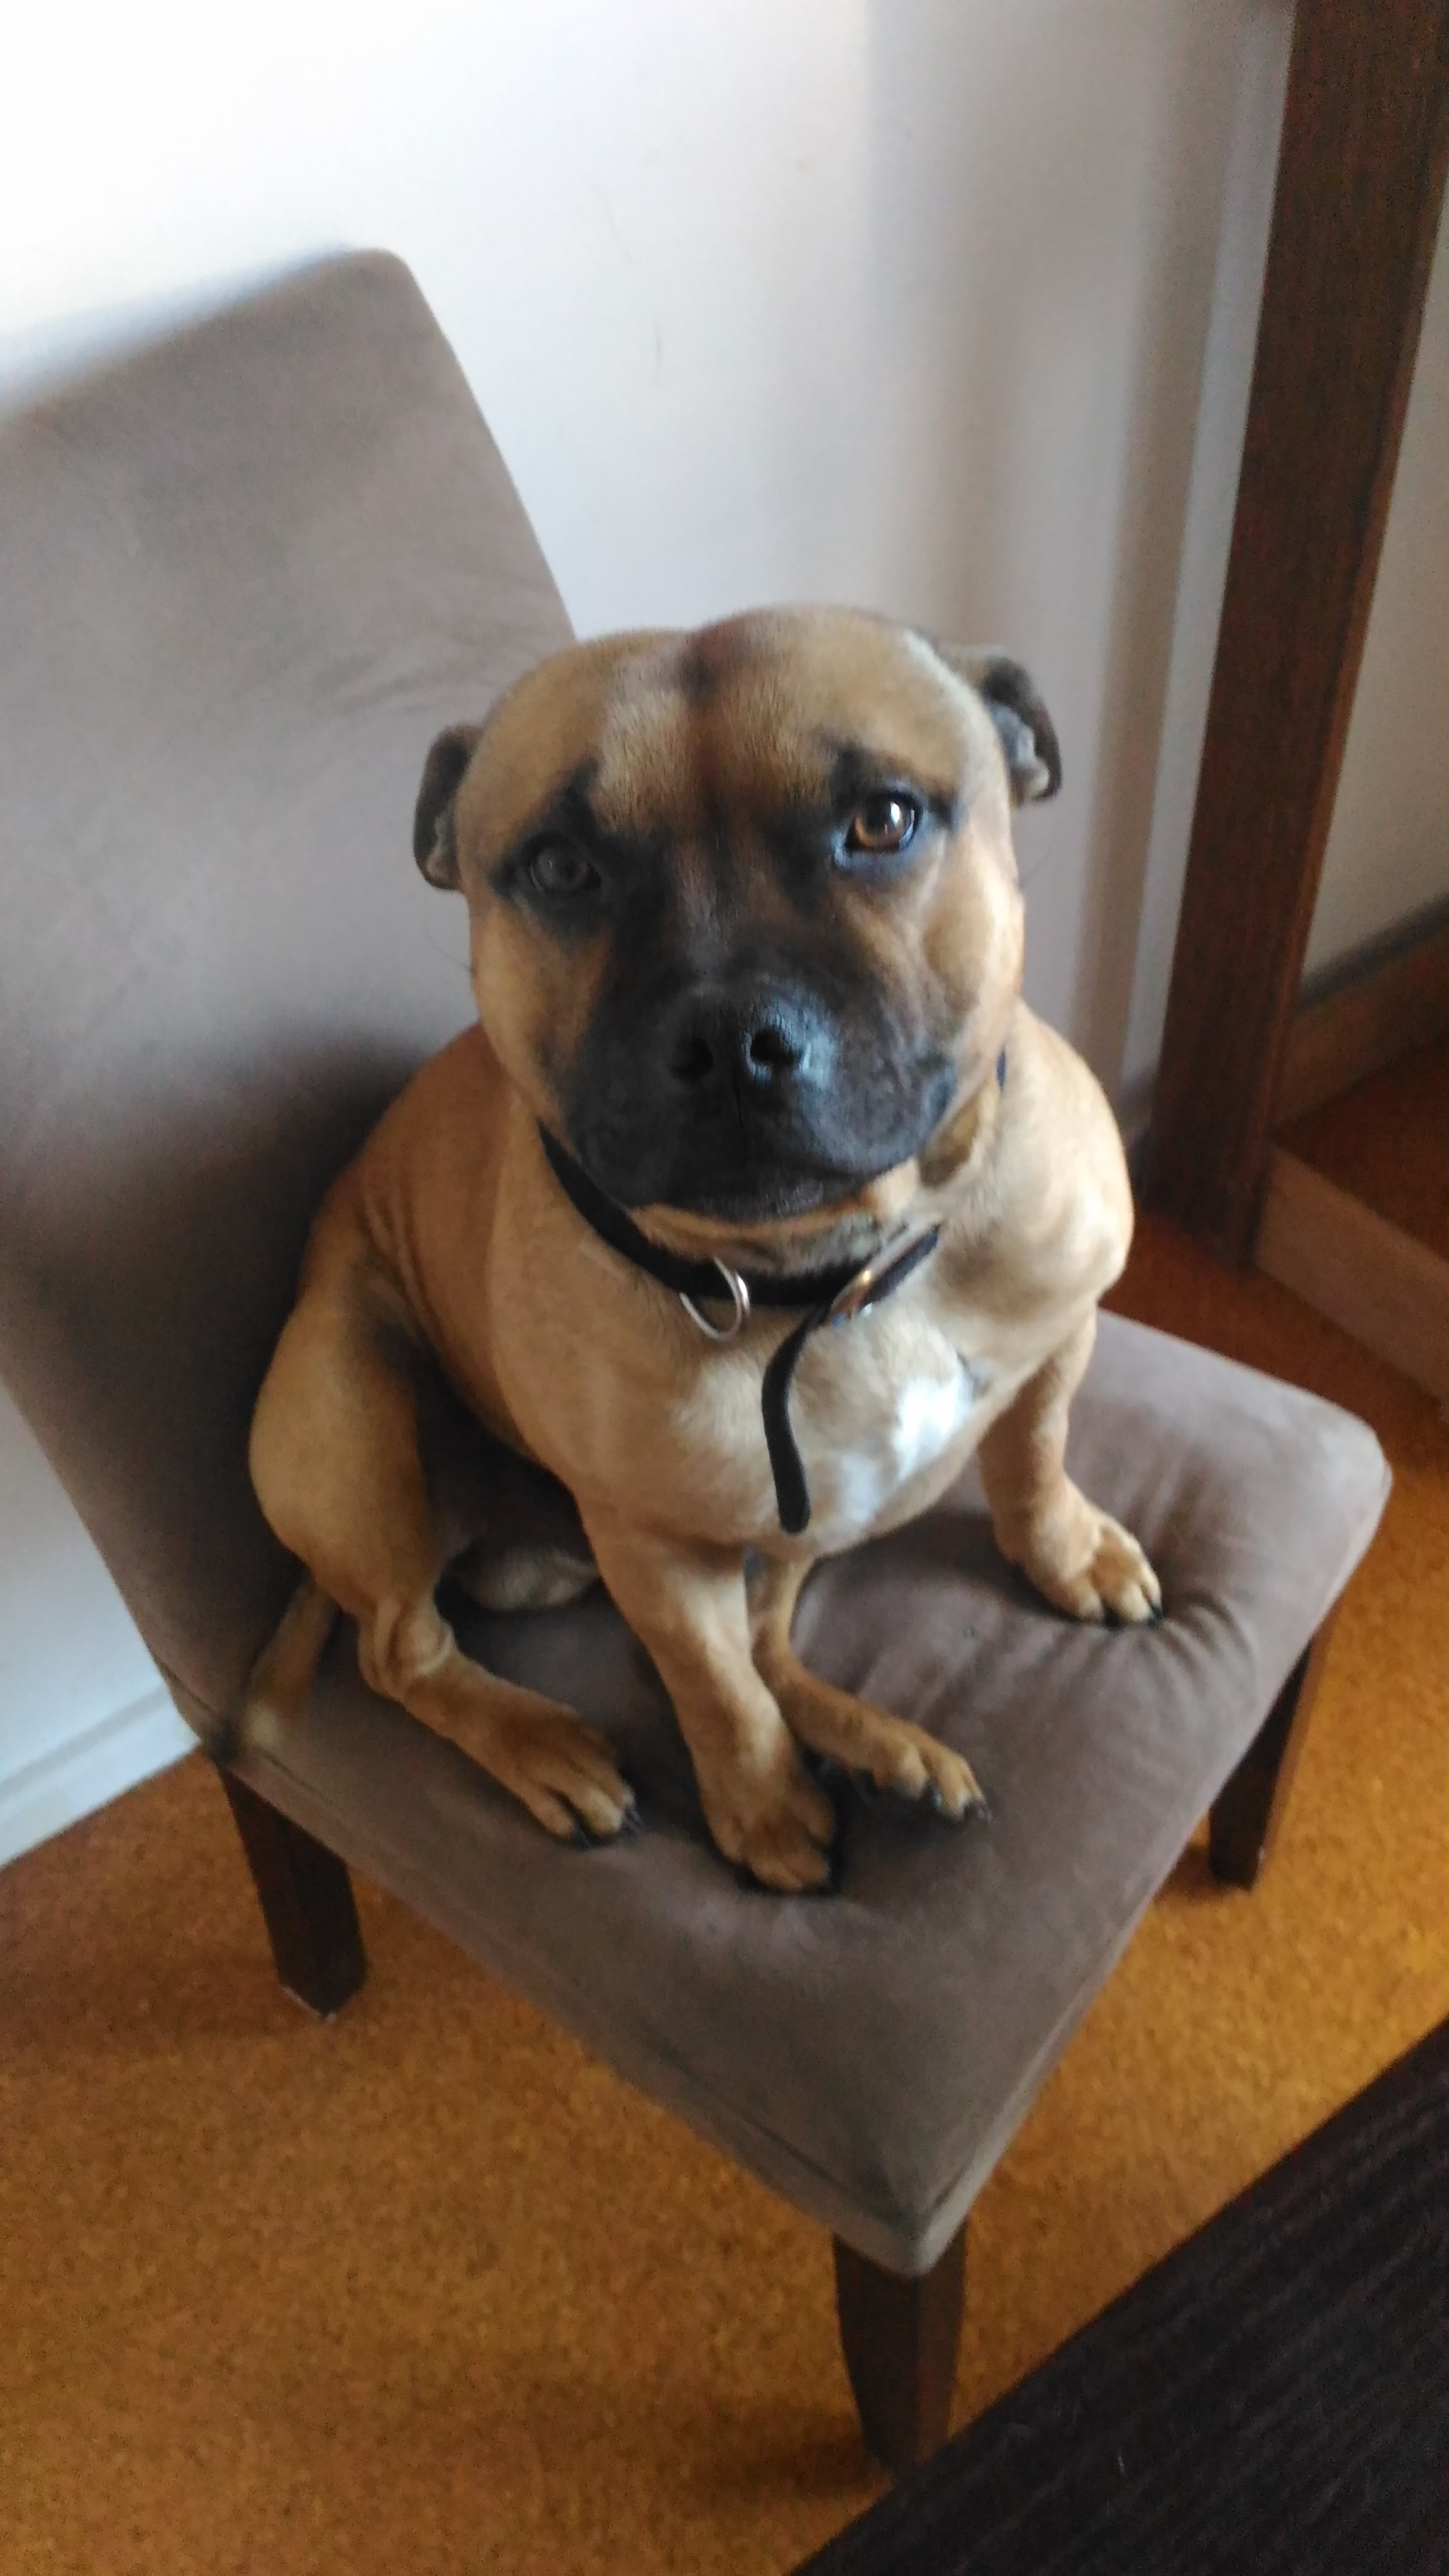
\includegraphics[width=30cm,height=30cm, keepaspectratio]{figs/turbo.jpg}
\end{figure}
 \end{center}
